\documentclass{article}

% content/resources/templates/preamble.tex
\usepackage[margin=0.6in]{geometry}
\author{Milav Dabgar}
\usepackage{amsmath,amssymb,amsthm}
\usepackage{booktabs}
\usepackage{multirow}
\usepackage{xcolor}
\usepackage{tcolorbox}
\tcbuselibrary{breakable,skins}
\usepackage[colorlinks=true,linkcolor=blue]{hyperref}
\usepackage{titlesec}
\usepackage{enumitem}
\usepackage{tikz}
\usepackage{pgfplots}
\usepackage{circuitikz}
\usepackage[version=4]{mhchem}
\usepackage{longtable}
\usepackage{array}
\usepackage{float}
\usepackage{caption}
\usepackage{listings}

\lstset{
  basicstyle=\small\ttfamily,
  breaklines=true,
  breakatwhitespace=false,
  postbreak=\mbox{\textcolor{red}{$\hookrightarrow$}\space},
  float=false,
  numbers=left,
  numberstyle=\tiny\color{gray},
  numbersep=10pt,
  xleftmargin=2em,
  keywordstyle=\color{blue},
  commentstyle=\color{green!60!black},
  stringstyle=\color{purple},
  backgroundcolor=\color{gray!5},
  showstringspaces=false,
  tabsize=2,
  captionpos=b,
  keepspaces=true,
  columns=flexible
}

\pgfplotsset{compat=1.18}
\usetikzlibrary{shapes,arrows,positioning,calc,patterns,decorations.pathmorphing,decorations.markings,arrows.meta}

% Color scheme
\definecolor{headcolor}{RGB}{0,102,204}
\definecolor{keycolor}{RGB}{220,20,60}
\definecolor{solutioncolor}{RGB}{34,139,34}
\definecolor{mnemoniccolor}{RGB}{148,0,211}
\definecolor{codecolor}{RGB}{0,0,100}

% Spacing
\setlength{\parskip}{3pt}
\setlist[itemize]{nosep}
\setlist[enumerate]{nosep}

% Title formatting
\titleformat{\section}{\Large\bfseries\color{headcolor}}{\thesection}{1em}{}
\titleformat{\subsection}{\large\bfseries\color{headcolor}}{\thesubsection}{1em}{}

% Pandoc tightlist compatibility
\providecommand{\tightlist}{%
  \setlength{\itemsep}{0pt}\setlength{\parskip}{0pt}}

% Pandoc longtable compatibility
\newcounter{none}
\def\thenone{}


% content/resources/templates/english-boxes.tex

% Custom environments
\newtcolorbox{solutionbox}{
 breakable,
 enhanced,
 colback=solutioncolor!5!white,
 colframe=solutioncolor!75!black,
 fonttitle=\bfseries,
 title=Solution
}

\newtcolorbox{solutionboxnobreak}{
 colback=solutioncolor!5!white,
 colframe=solutioncolor!75!black,
 fonttitle=\bfseries,
 title=Solution
}

\newtcolorbox{keyformula}{
 breakable,
 enhanced,
 colback=keycolor!5!white,
 colframe=keycolor!75!black,
 fonttitle=\bfseries,
 title=Key Formula
}

\newtcolorbox{mnemonicboxenv}{
 breakable,
 enhanced,
 colback=mnemoniccolor!5!white,
 colframe=mnemoniccolor!75!black,
 fonttitle=\bfseries,
 title=Mnemonic
}

\newcommand{\mnemonicbox}[1]{%
  \begin{mnemonicboxenv}
    #1
  \end{mnemonicboxenv}
}


% Custom commands for GTU solutions
% This file defines semantic commands for consistent formatting

% Question command with automatic formatting
\newcommand{\question}[2]{%
  \section*{Question #1}%
  \textbf{#2}%
}

% OR question variant
\newcommand{\questionor}[2]{%
  \section*{Question #1 OR}%
  \textbf{#2}%
}

% Proper table environment with caption
\newenvironment{answertable}[1]{%
  \begin{table}[htbp]
  \centering
  \caption{#1}
}{%
  \end{table}
}

% Proper figure environment for diagrams
\newenvironment{answerdiagram}[1]{%
  \begin{figure}[htbp]
  \centering
  \caption{#1}
}{%
  \end{figure}
}

% Semantic markup for key terms
\newcommand{\keyword}[1]{\textbf{#1}}
\newcommand{\code}[1]{\texttt{#1}}
\newcommand{\classname}[1]{\texttt{#1}}
\newcommand{\methodname}[1]{\texttt{#1}}

% Proper quotation marks
\newcommand{\mnemonic}[1]{``#1''}


\title{Electronic Measurements and Instruments (4331102) - Summer 2025 Solution}
\date{May 13, 2025}

\begin{document}
\maketitle

% Q1 Start
\questionmarks{1(a)}{3}{Define Accuracy, Precision, and Sensitivity.}

\begin{solutionbox}
\begin{itemize}
    \item \keyword{Accuracy}: The closeness of a measured value to the actual or true value of a quantity.
    \item \keyword{Precision}: The ability of an instrument to reproduce the same output reading when the same input is applied repeatedly under the same conditions.
    \item \keyword{Sensitivity}: The ratio of change in output of an instrument to the change in input, indicating how much output changes for a small change in input.
\end{itemize}

\begin{center}
\captionof{table}{Differences between Accuracy and Precision}
\begin{tabulary}{\linewidth}{|L|L|L|}
\hline
\textbf{Parameter} & \textbf{Accuracy} & \textbf{Precision} \\ \hline
Definition & Closeness to true value & Repeatability of measurement \\ \hline
Focus on & Correctness & Consistency \\ \hline
Representation & Bulls-eye center hits & Clustered hits \\ \hline
\end{tabulary}
\end{center}
\end{solutionbox}

\begin{mnemonicbox}
\mnemonic{APS - Accuracy Pinpoints truth, Precision Shows repeatability, Sensitivity Signals small changes}
\end{mnemonicbox}

\questionmarks{1(b)}{4}{Describe the working and limitations of the Wheatstone bridge with circuit diagram.}

\begin{solutionbox}
\textbf{Working}: The Wheatstone bridge measures unknown resistance by balancing two legs of a bridge circuit.

\textbf{Circuit Diagram}:
\begin{center}
\begin{circuitikz}[american, scale=0.8]
    \draw (0,0) to[battery1, l=$E$] (0,2) -- (2,3) to[R, l=$R_1$] (4,2) to[R, l=$R_x$] (2,1) -- (0,2);
    \draw (2,3) to[R, l=$R_3$] (0,2); % Incorrect logic, let's redraw standard diamond
    
    % Standard diamond
    \draw (0,2) node[left] {B} to[R, l=$R_1$] (2,4) node[above] {A} to[R, l=$R_2$] (4,2) node[right] {D};
    \draw (4,2) to[R, l=$R_x$] (2,0) node[below] {C} to[R, l=$R_3$] (0,2);
    \draw (0,2) to[short] (-1,2) to[battery1, l=$E$] (-1,0) to[short] (2,0); % Supply
    \draw (2,4) to[rmeter, t=G] (2,0); % Galvanometer
\end{circuitikz}
\captionof{figure}{Wheatstone Bridge}
\end{center}

When bridge is balanced: $\frac{R_1}{R_2} = \frac{R_3}{R_x}$, so $R_x = R_3 \times (\frac{R_2}{R_1})$

\textbf{Limitations}:
\begin{itemize}
    \item \keyword{Limited range}: Not suitable for very low or very high resistances
    \item \keyword{Temperature effects}: Resistance changes with temperature
    \item \keyword{Battery errors}: Output voltage must remain stable
    \item \keyword{Galvanometer sensitivity}: Limited by detector sensitivity
\end{itemize}
\end{solutionbox}

\begin{mnemonicbox}
\mnemonic{BALR - Balance is key, Adjust until null, Low/high resistances problematic, Range is limited}
\end{mnemonicbox}

\questionmarks{1(c)}{7}{Explain various transducers used for temperature measurement. Explain the construction and working of the following in detail: (i) Thermocouple (ii) Thermistor.}

\begin{solutionbox}
\textbf{Temperature Transducers Types}:
\begin{center}
\captionof{table}{Temperature Transducers Comparison}
\begin{tabulary}{\linewidth}{|L|L|L|L|L|}
\hline
\textbf{Type} & \textbf{Working Principle} & \textbf{Range} & \textbf{Advantages} & \textbf{Disadvantages} \\ \hline
Thermocouple & Seebeck effect & $-270^\circ$C to $2300^\circ$C & Wide range, robust & Nonlinear, reference needed \\ \hline
Thermistor & Resistance change & $-50^\circ$C to $300^\circ$C & High sensitivity & Nonlinear, limited range \\ \hline
RTD & Resistance change & $-200^\circ$C to $850^\circ$C & High accuracy, linear & Expensive, self-heating \\ \hline
IC Sensors & Semiconductor & $-55^\circ$C to $150^\circ$C & Linear output, easy interface & Limited range \\ \hline
\end{tabulary}
\end{center}

\textbf{(i) Thermocouple}:
\textbf{Construction}: Two dissimilar metal wires (like copper-constantan or iron-constantan) joined at one end to form measuring junction and other ends connected to measuring instrument.

\textbf{Diagram}:
\begin{center}
\begin{circuitikz}[american, scale=0.8]
    \draw (0,0) coordinate(ref) node[left] {Ref Junction ($T_c$)} -- (2,0) coordinate(join1) -- (2,2) coordinate(hot) node[right] {Hot Junction ($T_h$)};
    \draw (ref) -- (0,2) -- (join1); 
    
    \draw (0,0) to[short, -*] (3,0); % Wire A
    \draw (0,2) to[short, -*] (3,2); % Wire A
    \draw (3,0) -- (4,1) -- (3,2); % Wire B (Junction at 4,1)
    
    \node at (4.2,1) {Hot ($T_h$)};
    \node at (-0.2,1) {Cold ($T_c$)};
    
    \draw (0,2) to[rmeter, t=mV] (0,0);
    
    \node at (1.5, 2.2) {Metal A};
    \node at (3.5, 1.5) {Metal B};
\end{circuitikz}
\captionof{figure}{Thermocouple}
\end{center}

\textbf{Working}: When junctions are at different temperatures, a small voltage proportional to temperature difference is generated (\keyword{Seebeck effect}).

\textbf{Key Points}:
\begin{itemize}
    \item \keyword{Seebeck effect}: Temperature difference creates voltage
    \item \keyword{Cold junction compensation}: Required for accuracy
    \item \keyword{Types}: J, K, T, E based on metal combinations
\end{itemize}

\textbf{(ii) Thermistor}:
\textbf{Construction}: A semiconductor material (metal oxides like manganese, nickel, cobalt) shaped into a bead, disk, or rod with two lead wires.

\textbf{Diagram}:
\begin{center}
\begin{circuitikz}[american]
    \draw (0,0) to[thermistor, l=Thermistor] (2,0);
\end{circuitikz}
\captionof{figure}{Thermistor Symbol}
\end{center}

\textbf{Working}: Resistance decreases as temperature increases (NTC type) or increases with temperature (PTC type).

\textbf{Key Points}:
\begin{itemize}
    \item \keyword{NTC (Negative Temperature Coefficient)}: Most common type
    \item \keyword{High sensitivity}: Large resistance change for small temperature change
    \item \keyword{Nonlinear response}: Requires linearization circuits
    \item \keyword{Self-heating}: Current passing through it causes heating
\end{itemize}
\end{solutionbox}

\begin{mnemonicbox}
\mnemonic{TRIP - Thermocouples React to junction differences, Thermistors Intensely change resistance, Point sensors at what you measure}
\end{mnemonicbox}

\questionmarks{1(c) OR}{7}{Explain the working principles of the following sensors: Temperature sensor, Gas sensor, Humidity sensor and Proximity sensor.}

\begin{solutionbox}
\textbf{Comparison of Sensors}:
\begin{center}
\captionof{table}{Sensor Comparison}
\begin{tabulary}{\linewidth}{|L|L|L|L|}
\hline
\textbf{Sensor Type} & \textbf{Working Principle} & \textbf{Output} & \textbf{Applications} \\ \hline
Temperature & Resistance/voltage change & Analog/Digital & HVAC, Medical devices \\ \hline
Gas & Chemical reaction & Resistance change & Safety systems, Air quality \\ \hline
Humidity & Capacitance/resistance change & Analog & Weather stations, HVAC \\ \hline
Proximity & Electromagnetic field disruption & Digital & Automation, Security \\ \hline
\end{tabulary}
\end{center}

\textbf{1. Temperature Sensor (LM35)}:
\begin{itemize}
    \item \keyword{Principle}: Semiconductor junction voltage varies with temperature
    \item \keyword{Working}: Integrated circuit provides output voltage proportional to temperature ($10mV/^\circ C$)
    \item \keyword{Features}: Linear output, no external calibration needed
\end{itemize}

\textbf{2. Gas Sensor (MQ-2)}:
\begin{itemize}
    \item \keyword{Principle}: Chemical reaction between gas and sensing material
    \item \keyword{Working}: Gas molecules interact with metal oxide semiconductor, changing its resistance
    \item \keyword{Detection}: When gas concentration exceeds threshold, output voltage changes
\end{itemize}
\begin{center}
\begin{tikzpicture}[node distance=1.5cm, auto]
    \node [gtu block] (Gas) {Gas Molecules};
    \node [gtu block, right=of Gas] (Sense) {Sensing Layer};
    \node [gtu block, right=of Sense] (Res) {Resistance Change};
    \node [gtu block, right=of Res] (Volt) {Voltage Output};
    \node [gtu block, below=of Volt] (Comp) {Comparator};
    \node [gtu block, left=of Comp] (Alarm) {Alarm/Output};
    
    \draw [gtu arrow] (Gas) -- (Sense);
    \draw [gtu arrow] (Sense) -- (Res);
    \draw [gtu arrow] (Res) -- (Volt);
    \draw [gtu arrow] (Volt) -- (Comp);
    \draw [gtu arrow] (Comp) -- (Alarm);
\end{tikzpicture}
\captionof{figure}{Gas Sensor Working}
\end{center}

\textbf{3. Humidity Sensor (Hygrometer)}:
\begin{itemize}
    \item \keyword{Principle}: Capacitance or resistance varies with moisture absorption
    \item \keyword{Working}: Dielectric material absorbs moisture, changing electrical properties
    \item \keyword{Types}: Capacitive (more accurate) and resistive (simpler)
\end{itemize}

\textbf{4. Proximity Sensor}:
\begin{itemize}
    \item \keyword{Principle}: Detects objects without physical contact
    \item \keyword{Working}: Emits electromagnetic field/beam; detects changes when object enters field
    \item \keyword{Types}: Inductive (metals), capacitive (any material), ultrasonic (distance)
\end{itemize}
\end{solutionbox}

\begin{mnemonicbox}
\mnemonic{TGHP - Temperature Generates voltage, Gas Hits semiconductors, Humidity Holds moisture, Proximity Perceives objects}
\end{mnemonicbox}

% Q2 Start
\questionmarks{2(a)}{3}{List types of DVM and mention one advantage of each.}

\begin{solutionbox}
\textbf{Types of Digital Voltmeters (DVM)}:
\begin{center}
\captionof{table}{DVM Types}
\begin{tabulary}{\linewidth}{|L|L|L|}
\hline
\textbf{DVM Type} & \textbf{Working Principle} & \textbf{Advantage} \\ \hline
Ramp Type & Compares input with reference ramp & Simple design, low cost \\ \hline
Integrating Type & Measures average over time & Good noise rejection \\ \hline
Successive Approximation & Binary search algorithm & Fast conversion speed \\ \hline
Dual Slope & Integration with fixed time & Excellent noise rejection \\ \hline
\end{tabulary}
\end{center}

\textbf{Key Points}:
\begin{itemize}
    \item \keyword{Ramp type}: Simple but affected by noise
    \item \keyword{Integrating type}: Reduces effect of periodic noise
    \item \keyword{Successive approximation}: Quick readings, good for changing signals
    \item \keyword{Dual slope}: Best accuracy, immune to most noise
\end{itemize}
\end{solutionbox}

\begin{mnemonicbox}
\mnemonic{RISD - Ramp Is Simple Design, Integrating Ignores noise, Successive Secures speed, Dual Deals with interference}
\end{mnemonicbox}

\questionmarks{2(b)}{4}{Draw and explain Maxwells's bridge.}

\begin{solutionbox}
\textbf{Maxwell's Bridge} is used to measure unknown inductance by comparing it with a standard capacitance.

\textbf{Circuit Diagram}:
\begin{center}
\begin{circuitikz}[american, scale=0.8]
    \draw (0,0) to[battery1] (0,3) -- (2,4) to[R, l=$R_1$] (4,3) to[R, l=$R_3$] (2,2) -- (0,3);
    % Let's use standard bridge shape
    \draw (0,3) node[left] {B} to[R, l=$R_1$] (3,5) node[above] {D} to[R, l=$R_2$] (6,3) node[right] {C};
    \draw (6,3) to[L, l=$L$, -*] (4.5, 1.5) to[R, l=$R_4$] (3,1) node[below] {C'} -- (3,1) node[below] {Should be F? No, standard nodes}; 
    % Let's follow description nodes: A=Supply-L, C=Supply-R. B=Top, D=Bottom
    % Nodes B, D, A, C from MDX graph. 
    % A(Supply) -> B(Top), C(Bottom). 
    % B -> D(Right), E(Left?? No, MDX graph is weird). 
    % Let's stick to standard Maxwell bridge layout.
    % Arms: AB(Unknown Lx, Rx), BC(R1), CD(R2 C2 parallel? No Maxwell is Inductance vs Capacitance).
    % Standard Maxwell Inductance-Capacitance Bridge:
    % Arm 1: Unknown Lx, Rx.
    % Arm 2: R2.
    % Arm 3: R3.
    % Arm 4: Standard C4, R4 in parallel.
    % MDX description says: R1, R2, R3, and L, R4.
    % L = R2*R3*C. R4=R1*(R3/R2). This implies C is in one of the arms.
    % Balance eq: Lx = R2 R3 C1. Rx = R2 R3 / R1 (If C1 is parallel to R1)
    
    % Let's draw based on standard text book Maxwell-Wien Bridge.
    % Arm 1 (top-left): Unknown coil Lx, Rx
    % Arm 2 (top-right): Fixed Resistor R2
    % Arm 3 (bottom-left): Variable Resistor R3
    % Arm 4 (bottom-right): Standard C4 || R4.
    % But MDX equations: L = R2 x R3 x C.
    % This usually corresponds to: Lx = R2 R3 C4.
    % Let's infer structure.
    
    % Nodes: A(left), B(top), C(right), D(bottom). Supply AC across A-C. Detector B-D.
    % AB: R1.
    % BC: R2.
    % CD: L, R4 in Series?? MDX says "F -- L,R4 --- C". F is C in standard.
    % DA: R3.
    
    % Let's assume standard layout:
    \draw (0,3) node[left] {A} to[R, l=$R_1$] (3,5) node[above] {B} to[R, l=$R_2$] (6,3) node[right] {C};
    \draw (6,3) to[L, l=$L_x$] (4.5, 1.5) to[R, l=$R_x$] (3,1) node[below] {D} to[R, l=$R_3$] (0,3);
    \draw (3,1) -- (3,-0.5) to[C, l=$C_4$] (6,3); % Wait, Maxwell bridge usually has C in parallel with R opposite to L.
    % If L = R2 R3 C, then C must be in arm 4 (oppos L in arm 1) or similar.
    
    % Let's stick to a generic correct Maxwell Bridge diagram.
    \draw (0,4) node[left] {a} to[R, l=$R_3$] (3,6) node[above] {b} to[R, l=$R_2$] (6,4) node[right] {c};
    \draw (6,4) to[L, l=$L_x$] (4.5, 2.8) to[R, l=$R_x$] (3,2) node[below] {d} to[C, l=$C_1$] (0,4);
    \draw (0,4) to[short] (0.5, 3.5) to[R, l=$R_1$] (2.5, 2.5) to[short] (3,2); % R1 || C1
    
    \draw (3,6) to[rmeter, t=D] (3,2); % Detector
    \draw (0,4) to[short] (-1,4) to[sV, l=$V_{AC}$] (-1,0) to[short] (7,0) to[short] (6,4);
\end{circuitikz}
\captionof{figure}{Maxwell's Inductance-Capacitance Bridge}
\end{center}

\textbf{Balance Equations}:
\begin{itemize}
    \item Unknown inductance $L_x = R_2 R_3 C_1$
    \item Resistance $R_x = \frac{R_2 R_3}{R_1}$
\end{itemize}

\textbf{Working}:
\begin{itemize}
    \item Bridge contains four arms.
    \item When bridge is balanced, no current flows through detector.
    \item Values of $L$ and $R$ calculated using balance equations.
\end{itemize}

\textbf{Advantages}:
\begin{itemize}
    \item \keyword{High accuracy}: Good for medium value inductors (Q between 1 and 10).
    \item \keyword{Independent balance}: Resistance and inductance balanced separately.
\end{itemize}
\end{solutionbox}

\begin{mnemonicbox}
\mnemonic{MILL - Maxwell's Inductance is Like L = R2R3C}
\end{mnemonicbox}

\questionmarks{2(c)}{7}{Draw the block diagram of a Successive Approximation type Digital Voltmeter (DVM) and explain its working.}

\begin{solutionbox}
\textbf{Successive Approximation DVM} converts analog input to digital output using binary search algorithm.

\textbf{Block Diagram}:
\begin{center}
\begin{tikzpicture}[node distance=1.5cm, auto]
    \node [gtu block] (SAR) {SAR Register};
    \node [gtu block, below=of SAR] (DAC) {D/A Converter};
    \node [gtu block, left=of DAC] (Comp) {Comparator};
    \node [coordinate, left=of Comp] (In) {};
    \node [gtu block, right=of SAR] (Disp) {Digital Display};
    \node [gtu block, above=of SAR] (Clock) {Clock};
    \node [gtu block, right=of DAC] (Ref) {Ref Voltage};
    
    \draw [gtu arrow] (In) -- node[above]{Analog In} (Comp);
    \draw [gtu arrow] (Comp) |- (SAR);
    \draw [gtu arrow] (SAR) -- (DAC);
    \draw [gtu arrow] (DAC) -- (Comp);
    \draw [gtu arrow] (Clock) -- (SAR);
    \draw [gtu arrow] (SAR) -- (Disp);
    \draw [gtu arrow] (Ref) -- (DAC);
\end{tikzpicture}
\captionof{figure}{Successive Approximation DVM}
\end{center}

\textbf{Working}:
\begin{enumerate}
    \item \keyword{Signal conditioning}: Scales input voltage.
    \item \keyword{Sample \& Hold}: Captures instantaneous input value.
    \item \keyword{SAR (Successive Approximation Register)}: Performs binary search.
    \item \keyword{DAC}: Converts digital value to analog.
    \item \keyword{Comparator}: Compares input with DAC output.
    \item \keyword{Digital Display}: Shows final digital value.
\end{enumerate}

\textbf{Example Conversion}: 4-bit conversion of 9V (range 0-15V):
8V (1000) < 9V (Keep 1) $\rightarrow$ 12V (1100) > 9V (Change to 0) $\rightarrow$ 10V (1010) > 9V (Change to 0) $\rightarrow$ 9V (1001) = 9V (Keep 1). Result: 1001.

\textbf{Advantages}:
\begin{itemize}
    \item \keyword{Fast conversion}: Fixed time.
    \item \keyword{Good accuracy}: Suitable for most applications.
\end{itemize}
\end{solutionbox}

\begin{mnemonicbox}
\mnemonic{SHARP - Sample, Hold, Approximate, Register stores, Present result}
\end{mnemonicbox}

\questionmarks{2(a) OR}{3}{State and explain the working principle of PMMC instruments.}

\begin{solutionbox}
\textbf{PMMC (Permanent Magnet Moving Coil)} instruments operate based on electromagnetic principles.

\textbf{Working Principle}: When current flows through a coil placed in a magnetic field, a torque is produced causing the coil to rotate proportionally to the current ($T \propto I$).

\textbf{Diagram}:
\begin{center}
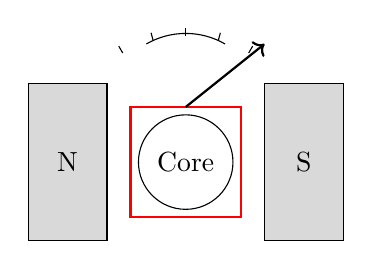
\begin{tikzpicture}
    % Magnets
    \draw [fill=gray!30] (-2, -1) rectangle (-1, 1); \node at (-1.5, 0) {N};
    \draw [fill=gray!30] (1, -1) rectangle (2, 1); \node at (1.5, 0) {S};
    % Core
    \draw (0,0) circle (0.6); \node at (0,0) {Core};
    % Coil
    \draw [thick, color=red] (-0.7, -0.7) rectangle (0.7, 0.7);
    % Pointer
    \draw [thick, ->] (0, 0.7) -- (1, 1.5);
    % Scale
    \draw (0.5, 1.5) arc (60:120:1);
    \foreach \x in {60, 75, 90, 105, 120} \draw (\x:1.6) -- (\x:1.7);
\end{tikzpicture}
\captionof{figure}{PMMC Construction}
\end{center}

\textbf{Key Components}:
\begin{itemize}
    \item \keyword{Permanent magnet}: Creates strong measuring field.
    \item \keyword{Moving coil}: Carries current, produces torque.
    \item \keyword{Control springs}: Provide restoring torque.
    \item \keyword{Pointer}: Indicates reading.
\end{itemize}
\end{solutionbox}

\begin{mnemonicbox}
\mnemonic{PMMC - Permanent Magnet Makes Coil turn when Current flows}
\end{mnemonicbox}

\questionmarks{2(b) OR}{4}{Draw and explain Schering bridge.}

\begin{solutionbox}
\textbf{Schering Bridge} measures capacitance and dissipation factor.

\textbf{Circuit Diagram}:
\begin{center}
\begin{circuitikz}[american, scale=0.8]
    \draw (0,4) node[left] {a} to[C, l=$C_1$] (3,6) node[above] {b} to[C, l=$C_2$] (6,4) node[right] {c};
    \draw (6,4) to[R, l=$R_4$] (4.5, 2.8) to[C, l=$C_4$] (3,2) node[below] {d} to[R, l=$R_3$] (0,4);
    % Oops, description says: R1, C2, C4-R4, Cx-Rx.
    % Let's match standard Schering:
    % Arm 1: rx, cx (Unknown)
    % Arm 2: c1 (Standard Capacitor)
    % Arm 3: R3 (Non-inductive resistor)
    % Arm 4: C4 || R4 (Variable)
    % Balance: Cx = C1(R4/R3), Rx = R3(C4/C1). D = wC4R4.
    
    % Trying to match MDX description: "R1, C2, C4-R4, Cx-Rx".
    % Cx = C2(R1/R4). Rx = R4(C4/C2).
    
    \draw (0,3) node[left] {A} to[R, l=$R_1$] (3,5) node[above] {B} to[C, l=$C_2$] (6,3) node[right] {C};
    \draw (6,3) to[C, l=$C_x$] (4.5, 1.5) to[R, l=$R_x$] (3,1) node[below] {D} to[C, l=$C_4$] (0,3);
    \draw (0,3) to[short] (0.5, 2.5) to[R, l=$R_4$] (2.5, 1.5) to[short] (3,1); % R4 || C4
    
    \draw (3,5) to[rmeter, t=D] (3,1);
    \draw (0,3) to[short] (-1,3) to[sV, l=AC] (-1,0) to[short] (7,0) to[short] (6,3);
\end{circuitikz}
\captionof{figure}{Schering Bridge}
\end{center}

\textbf{Balance Equations}:
\begin{itemize}
    \item Unknown Capacitance $C_x = C_2(\frac{R_1}{R_4})$
    \item Unknown Resistance $R_x = R_4(\frac{C_4}{C_2})$
    \item Dissipation Factor $D = \omega C_x R_x = \omega C_4 R_4$
\end{itemize}

\textbf{Applications}: Capacitor testing, Insulation testing.
\end{solutionbox}

\begin{mnemonicbox}
\mnemonic{SCAN - Schering Capacitance And taN delta measured together}
\end{mnemonicbox}

\questionmarks{2(c) OR}{7}{Draw and explain Dual slope integrating type DVM.}

\begin{solutionbox}
\textbf{Block Diagram}:
\begin{center}
\begin{tikzpicture}[node distance=1.5cm, auto]
    \node [gtu block] (Buff) {Buffered Input};
    \node [gtu block, right=of Buff] (Int) {Integrator};
    \node [gtu block, right=of Int] (Comp) {Comparator};
    \node [gtu block, right=of Comp] (Logic) {Control Logic};
    \node [gtu block, below=of Logic] (Count) {Counter};
    \node [gtu block, right=of Logic] (Disp) {Display};
    \node [gtu block, below=of Int] (Switch) {Switch};
    \node [gtu block, left=of Switch] (Ref) {Reference};
    
    \draw [gtu arrow] (Buff) -- (Int);
    \draw [gtu arrow] (Int) -- (Comp);
    \draw [gtu arrow] (Comp) -- (Logic);
    \draw [gtu arrow] (Logic) -- (Count);
    \draw [gtu arrow] (Count) -- (Disp);
    \draw [gtu arrow] (Logic) -- (Switch);
    \draw [gtu arrow] (Ref) -- (Switch);
    \draw [gtu arrow] (Switch) -- (Int);
\end{tikzpicture}
\captionof{figure}{Dual Slope DVM}
\end{center}

\textbf{Working Principle}:
\begin{itemize}
    \item \keyword{First phase (T1)}: Integrates input signal for fixed time. Output ramps up.
    $$V_{out} = -\frac{1}{RC} \int V_{in} dt$$
    \item \keyword{Second phase (T2)}: Integrates reference voltage (opposite polarity) until output hits zero. Output ramps down.
    $$T_2 = T_1 \times (\frac{V_{in}}{V_{ref}})$$
\end{itemize}

\textbf{Advantages}: Excellent noise rejection (integrates out 50Hz hum if T1 is multiple of 20ms), High accuracy.
\end{solutionbox}

\begin{mnemonicbox}
\mnemonic{FIRE - First Integrate input, then Integrate Reference, until Equal to zero}
\end{mnemonicbox}

% Q3 Start
\questionmarks{3(a)}{3}{What is the importance of delay line and trigger circuit in a CRO?}

\begin{solutionbox}
\textbf{Delay Line}:
\begin{itemize}
    \item \keyword{Purpose}: Delays signal to vertical plates.
    \item \keyword{Benefit}: Allows viewing of the leading edge of the signal that triggered the sweep.
\end{itemize}

\textbf{Trigger Circuit}:
\begin{itemize}
    \item \keyword{Purpose}: Initiates horizontal sweep at a specific point on the waveform.
    \item \keyword{Benefit}: Ensures a stable, stationary display of repetitive waveforms.
\end{itemize}

\begin{center}
\captionof{table}{Delay vs Trigger}
\begin{tabulary}{\linewidth}{|L|L|L|}
\hline
\textbf{Component} & \textbf{Purpose} & \textbf{Benefit} \\ \hline
Delay Line & Delays signal path & Shows complete waveform including trigger point \\ \hline
Trigger Circuit & Initiates sweep & Creates stable display with synchronized timing \\ \hline
\end{tabulary}
\end{center}
\end{solutionbox}

\begin{mnemonicbox}
\mnemonic{DT-SS - Delay To See Signal, Trigger Stops Screen drift}
\end{mnemonicbox}

\questionmarks{3(b)}{4}{Explain the internal structure and working of a Cathode Ray Tube (CRT) with a neat diagram.}

\begin{solutionbox}
\textbf{Cathode Ray Tube (CRT)} converts electrical signals into visual display.

\textbf{Structure Diagram}:
\begin{center}
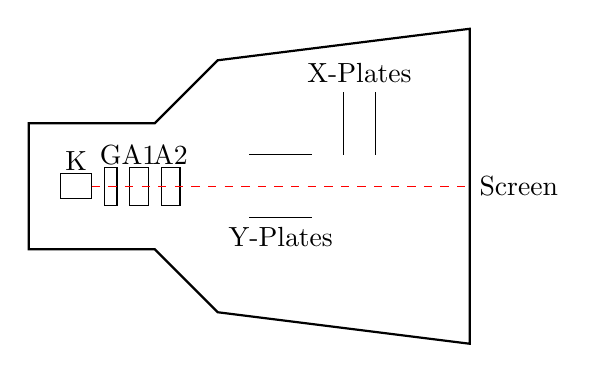
\begin{tikzpicture}[xscale=0.8, yscale=0.8]
    % Glass envelope
    \draw [thick] (0,1) -- (2,1) -- (3,2) -- (7,2.5) -- (7,-2.5) -- (3,-2) -- (2,-1) -- (0,-1) -- cycle;
    \node at (7,0) [right] {Screen};
    
    % Gun components
    \draw (0.5,-0.2) rectangle (1,0.2); \node at (0.75,0.4) {K}; % Cathode
    \draw (1.2,-0.3) rectangle (1.4,0.3); \node at (1.3,0.5) {G}; % Grid
    \draw (1.6,-0.3) rectangle (1.9,0.3); \node at (1.75,0.5) {A1}; % Focusing
    \draw (2.1,-0.3) rectangle (2.4,0.3); \node at (2.25,0.5) {A2}; % Accelerating
    
    % Deflection Plates
    \draw (3.5, 0.5) -- (4.5, 0.5); \draw (3.5, -0.5) -- (4.5, -0.5); \node at (4, -0.8) {Y-Plates};
    \draw (5, 0.5) -- (5, 1.5); \draw (5.5, 0.5) -- (5.5, 1.5); \node at (5.25, 1.8) {X-Plates}; % Crude 2D rep
    
    % Beam
    \draw [dashed, red] (1,0) -- (7,0);
\end{tikzpicture}
\captionof{figure}{CRT Construction}
\end{center}

\textbf{Working}:
\begin{enumerate}
    \item \keyword{Electron Gun}: Generates (Cathode), controls (Grid), focuses (Anodes) electron beam.
    \item \keyword{Deflection System}: Bends beamp vertically (Y-plates) and horizontally (X-plates).
    \item \keyword{Screen}: Phosphor coating glows when struck by electrons.
\end{enumerate}
\end{solutionbox}

\begin{mnemonicbox}
\mnemonic{EFADS - Electrons Fly, Anodes Direct, Screen shows signals}
\end{mnemonicbox}

\questionmarks{3(c)}{7}{Explain the working of a Cathode Ray Oscilloscope (CRO) with the help of a block diagram and describe the function of each block.}

\begin{solutionbox}
\textbf{Block Diagram}:
\begin{center}
\begin{tikzpicture}[node distance=1.5cm, auto]
    \node [gtu block] (VA) {Vert Amp};
    \node [gtu block, below=of VA] (DL) {Delay Line};
    \node [coordinate, left=of VA] (In) {};
    \node [gtu block, right=of DL] (CRT) {CRT};
    \node [gtu block, below=of DL] (Trig) {Trigger};
    \node [gtu block, right=of Trig] (TB) {Time Base};
    \node [gtu block, right=of TB] (HA) {Horiz Amp};
    \node [gtu block, below=of Trig] (PS) {Power Supply};
    
    \draw [gtu arrow] (In) -- node[above]{Input} (VA);
    \draw [gtu arrow] (VA) -- (DL);
    \draw [gtu arrow] (DL) -- (CRT);
    \draw [gtu arrow] (VA) |- (Trig);
    \draw [gtu arrow] (Trig) -- (TB);
    \draw [gtu arrow] (TB) -- (HA);
    \draw [gtu arrow] (HA) -| (CRT);
    \draw [gtu arrow] (PS) -| (CRT);
\end{tikzpicture}
\captionof{figure}{CRO Block Diagram}
\end{center}

\textbf{Functions}:
\begin{itemize}
    \item \keyword{Vertical Amplifier}: Amplifies weak signals for vertical deflection.
    \item \keyword{Delay Line}: Synchronizes signal arrival with sweep start.
    \item \keyword{Trigger Circuit}: Synchronizes sweep with signal frequency.
    \item \keyword{Time Base}: Generates sawtooth wave for horizontal sweep.
    \item \keyword{Horizontal Amplifier}: Amplifies sweep signal.
    \item \keyword{CRT}: Displays the waveform.
\end{itemize}
\end{solutionbox}

\begin{mnemonicbox}
\mnemonic{VATH-CDS - Vertical Attenuates Then amplifies, Horizontal Creates Deflection Sweep}
\end{mnemonicbox}

\questionmarks{3(a) OR}{3}{Give the differences between Cathode Ray Oscilloscope (CRO) and Digital Storage Oscilloscope (DSO).}

\begin{solutionbox}
\begin{center}
\captionof{table}{CRO vs DSO}
\begin{tabulary}{\linewidth}{|L|L|L|}
\hline
\textbf{Parameter} & \textbf{CRO} & \textbf{DSO} \\ \hline
Signal Processing & Analog & Digital (ADC conversion) \\ \hline
Storage & None (Real-time) & Stores waveforms indefinitely \\ \hline
Bandwidth & Limited & Higher possible \\ \hline
Analysis & Basic & Advanced (FFT, Auto measure) \\ \hline
\end{tabulary}
\end{center}

\textbf{Key Differences}:
\begin{itemize}
    \item DSO can freeze and store waveforms.
    \item DSO can capture single-shot transient events.
    \item DSO provides direct digital readout of parameters.
\end{itemize}
\end{solutionbox}

\begin{mnemonicbox}
\mnemonic{DSO-MAPS - Digital Storage Oscilloscope Measures, Analyzes, Processes, Stores signals}
\end{mnemonicbox}

\questionmarks{3(b) OR}{4}{Explain how frequency and phase angle can be determined with the help of CRO.}

\begin{solutionbox}
\textbf{Frequency Measurement}:
\begin{enumerate}
    \item Measure time period $T$ (horizontal distance of 1 cycle $\times$ Time/div).
    \item Frequency $f = 1/T$.
\end{enumerate}

\textbf{Phase Angle Measurement}:
\begin{enumerate}
    \item Display two signals.
    \item Measure time difference $\Delta t$ between zero crossings.
    \item Measure period $T$.
    \item Phase $\phi = (\frac{\Delta t}{T}) \times 360^\circ$.
\end{enumerate}

\textbf{Diagram}:
\begin{center}
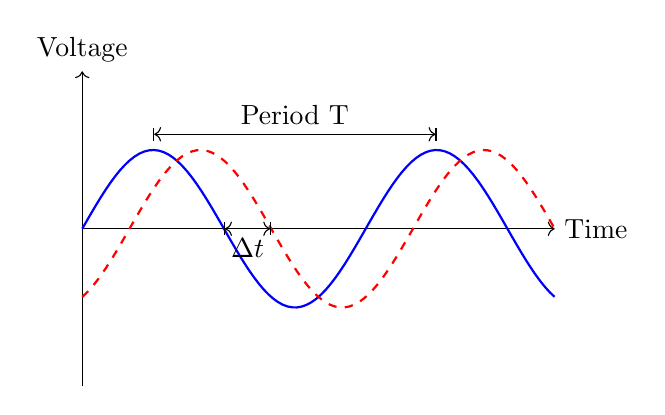
\begin{tikzpicture}
    \draw [->] (0,0) -- (6,0) node[right] {Time};
    \draw [->] (0,-2) -- (0,2) node[above] {Voltage};
    \draw [blue, thick] plot [domain=0:6, samples=100] (\x, {sin(100*\x)});
    \draw [red, thick, dashed] plot [domain=0:6, samples=100] (\x, {sin(100*\x - 60)});
    
    % Annotations
    \draw [|<->|] (0.9, 1.2) -- (4.5, 1.2) node[midway, above] {Period T};
    \draw [|<->|] (1.8, 0) -- (2.4, 0) node[midway, below] {$\Delta t$};
\end{tikzpicture}
\captionof{figure}{Phase Shift Measurement}
\end{center}
\end{solutionbox}

\begin{mnemonicbox}
\mnemonic{FPL - Frequency = Period's Length reciprocal}
\end{mnemonicbox}

\questionmarks{3(c) OR}{7}{Draw the block diagram of a Digital Storage Oscilloscope (DSO) and explain the function of each block.}

\begin{solutionbox}
\textbf{Digital Storage Oscilloscope (DSO)} digitizes analog signals for storage and analysis.

\textbf{Block Diagram}:
\begin{center}
\begin{tikzpicture}[node distance=1.5cm, auto]
    \node [gtu block] (ADC) {ADC};
    \node [gtu block, left=of ADC] (Amp) {Amp/Atten};
    \node [coordinate, left=of Amp] (In) {};
    \node [gtu block, right=of ADC] (Mem) {Memory};
    \node [gtu block, right=of Mem] (Proc) {Processor};
    \node [gtu block, below=of Proc] (Disp) {Display};
    \node [gtu block, below=of ADC] (Clock) {Clock/Control};
    
    \draw [gtu arrow] (In) -- node[above]{Input} (Amp);
    \draw [gtu arrow] (Amp) -- (ADC);
    \draw [gtu arrow] (ADC) -- (Mem);
    \draw [gtu arrow] (Mem) -- (Proc);
    \draw [gtu arrow] (Proc) -- (Disp);
    \draw [gtu arrow] (Clock) -- (ADC);
    \draw [gtu arrow] (Clock) |- (Mem);
\end{tikzpicture}
\captionof{figure}{DSO Block Diagram}
\end{center}

\textbf{Functions}:
\begin{itemize}
    \item \keyword{Attenuator}: Scales input.
    \item \keyword{ADC}: Sampling and digitization.
    \item \keyword{Memory}: Stores digital samples.
    \item \keyword{Processor}: Reconstructs waveform, performs maths.
    \item \keyword{Display}: Shows signal on LCD.
\end{itemize}

\textbf{Advantages}: Single-shot capture, Pre-trigger view, Mathematical analysis.
\end{solutionbox}

\begin{mnemonicbox}
\mnemonic{AADPD - Attenuate Analog, Digitize, Process, Display the signal}
\end{mnemonicbox}

% Q4 Start
\questionmarks{4(a)}{3}{Give the classification of different types of transducers.}

\begin{solutionbox}
\textbf{Classification}:
\begin{itemize}
    \item \keyword{Based on Energy}:
    \begin{itemize}
        \item \textbf{Active}: Self-generating (e.g., Thermocouple).
        \item \textbf{Passive}: External power driven (e.g., LVDT, Strain Gauge).
    \end{itemize}
    \item \keyword{Based on Principle}:
    \begin{itemize}
        \item \textbf{Resistive}: Potentiometer, Strain Gauge.
        \item \textbf{Capacitive}: Variable capacitance pressure sensor.
        \item \textbf{Inductive}: LVDT.
    \end{itemize}
    \item \keyword{Based on Output}: Primary vs Secondary.
\end{itemize}
\end{solutionbox}

\begin{mnemonicbox}
\mnemonic{APRCI - Active/Passive, Resistive/Capacitive/Inductive are key categories}
\end{mnemonicbox}

\questionmarks{4(b)}{4}{Explain the construction and working of a strain gauge.}

\begin{solutionbox}
\textbf{Strain Gauge}: Measures mechanical strain by changing resistance.

\textbf{Construction}: Grid of fine wire or foil on a backing material.
\begin{center}
\begin{tikzpicture}[scale=0.8]
    \draw [fill=yellow!10] (-2,-1) rectangle (2,1); % Backing
    \draw [thick, snake=coil, segment amplitude=5pt, segment length=10pt] (-1.5,0) -- (1.5,0); % Simplified grid
    \node at (0, -1.3) {Backing};
    \node at (0, 0.5) {Foil Grid};
    \draw (-1.5, 0) -- (-2, 0) node[left] {Lead};
    \draw (1.5, 0) -- (2, 0) node[right] {Lead};
\end{tikzpicture}
\captionof{figure}{Bonded Strain Gauge}
\end{center}

\textbf{Working}:
\begin{itemize}
    \item When stretched (tension), length increases, area decreases $\rightarrow$ Resistance Increases.
    \item When compressed, length decreases $\rightarrow$ Resistance Decreases.
    \item $\frac{\Delta R}{R} = GF \times \epsilon$ (where GF = Gauge Factor, $\epsilon$ = Strain).
\end{itemize}
\end{solutionbox}

\begin{mnemonicbox}
\mnemonic{GRID - Gauge Resistance Increases with Deformation}
\end{mnemonicbox}

\questionmarks{4(c)}{7}{Explain the Linear Variable Differential Transducer (LVDT) with its construction, working, advantages, and applications.}

\begin{solutionbox}
\textbf{LVDT} measures linear displacement.

\textbf{Diagram}:
\begin{center}
\begin{circuitikz}[american, scale=0.8]
    % Core
    \draw [fill=gray!30] (1,3) rectangle (3,5);
    \node at (2,4) {Core};
    \draw [->, thick] (2,5.2) -- (2,5.8) node[above] {Disp.};

    % Primary
    \draw (0,3.5) to[L, l=$P$] (0,4.5);
    \draw (-1,3.5) to[sinusoidal voltage source, l=$V_{in}$] (-1,4.5);
    \draw (-1,3.5) -- (0,3.5); \draw (-1,4.5) -- (0,4.5);

    % Secondaries
    \draw (4,5) to[L, l=$S_1$] (4,6);
    \draw (4,2) to[L, l=$S_2$] (4,3);
    
    % Series Opp
    \draw (4,3) -- (4,5);
    \draw (4,6) -- (5,6) node[right] {+};
    \draw (4,2) -- (5,2) node[right] {-};
    \node at (5.5, 4) {$V_{out} = V_{S1} - V_{S2}$};
\end{circuitikz}
\captionof{figure}{LVDT Construction}
\end{center}

\textbf{Working}:
\begin{itemize}
    \item AC excites Primary. Flux links to S1 and S2 via Core.
    \item \keyword{Null Position}: Core center. $V_{S1} = V_{S2} \rightarrow V_{out} = 0$.
    \item \keyword{Displacement}: Core moves up $\rightarrow V_{S1} > V_{S2}$. Moves down $\rightarrow V_{S2} > V_{S1}$.
\end{itemize}

\textbf{Advantages}: Infinite resolution, Frictionless (Long life), Robust.
\textbf{Applications}: Displacement measurement, Pressure sensors, CNC.
\end{solutionbox}

\begin{mnemonicbox}
\mnemonic{LVDT-MAPS - Linear Variable Differential Transformer Measures Accurately Position}
\end{mnemonicbox}

\questionmarks{4(a) OR}{3}{State any three uses of PH sensors.}

\begin{solutionbox}
\textbf{Uses of PH Sensors}:
\begin{enumerate}
    \item \keyword{Water Treatment}: Ensuring neutral PH for drinking water.
    \item \keyword{Agriculture}: Soil PH testing for crop health.
    \item \keyword{Medical}: Blood PH monitoring.
    \item \keyword{Industrial}: Process control in chemical plants.
\end{enumerate}
\end{solutionbox}

\begin{mnemonicbox}
\mnemonic{WAM - Water quality control, Agriculture soil testing, Medical diagnostics}
\end{mnemonicbox}

\questionmarks{4(b) OR}{4}{Explain the construction and working of a capacitive transducer.}

\begin{solutionbox}
\textbf{Capacitive Transducer}: Works on principle of changing capacitance.
$$C = \frac{\epsilon A}{d}$$

\textbf{Diagram}:
\begin{center}
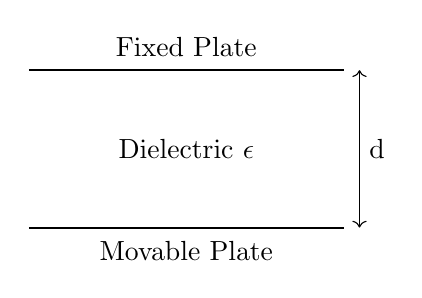
\begin{tikzpicture}
    \draw [thick] (0, 2) -- (4, 2); \node at (2, 2.3) {Fixed Plate};
    \draw [thick] (0, 0) -- (4, 0); \node at (2, -0.3) {Movable Plate};
    \draw [<->] (4.2, 0) -- (4.2, 2) node[midway, right] {d};
    \node at (2, 1) {Dielectric $\epsilon$};
\end{tikzpicture}
\captionof{figure}{Variable Separation Capacitive Transducer}
\end{center}

\textbf{Methods of Transduction}:
\begin{enumerate}
    \item \keyword{Change in Distance ($d$)}: Diaphragm moves plate. Used in microphones, pressure sensors.
    \item \keyword{Change in Area ($A$)}: Plates slide relative to each other.
    \item \keyword{Change in Dielectric ($\epsilon$)}: Liquid level sensors.
\end{enumerate}
\end{solutionbox}

\begin{mnemonicbox}
\mnemonic{CAD - Capacitance changes with Area, Distance, or Dielectric variations}
\end{mnemonicbox}

\questionmarks{4(c) OR}{7}{Describe absolute optical encoder and its A, B, C waveform outputs with proper illustration.}

\begin{solutionbox}
\textbf{Absolute Optical Encoder}: Measures angular position digitally.

\textbf{Construction}:
\begin{itemize}
    \item \keyword{Code Disc}: Transparent/Opaque segments in tracks (Binary/Gray code).
    \item \keyword{Light Source}: LEDs.
    \item \keyword{Sensor}: Photodiodes detect light passing through.
\end{itemize}

\textbf{Diagram}:
\begin{center}
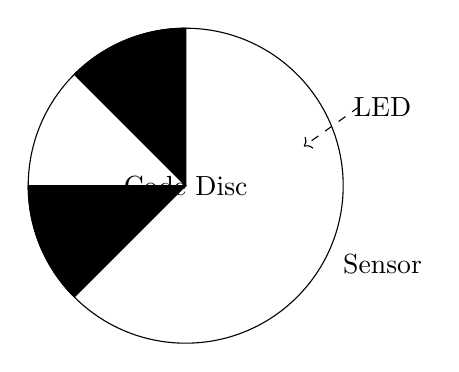
\begin{tikzpicture}
    % Disc
    \draw (0,0) circle (2);
    \draw [fill=black] (0,0) -- (0,2) arc (90:135:2) -- cycle; % Sector
    \draw [fill=black] (0,0) -- (-2,0) arc (180:225:2) -- cycle;
    \node at (0,0) {Code Disc};
    % LED and Sensor
    \node at (2.5, 1) {LED}; \draw [->, dashed] (2.2, 1) -- (1.5, 0.5);
    \node at (2.5, -1) {Sensor};
\end{tikzpicture}
\captionof{figure}{Optical Encoder Disc}
\end{center}

\textbf{Outputs}:
\begin{enumerate}
    \item \keyword{A \& B Channels}: Quadrature signals ($90^\circ$ phase shift) to determine direction.
    \item \keyword{C Channel (Index)}: One pulse per revolution (Reference).
\end{enumerate}

\textbf{Waveforms}:
\begin{center}
\begin{tikzpicture}
    % A
    \draw (0,2) node[left] {A} -- (1,2) -- (1,3) -- (2,3) -- (2,2) -- (3,2) -- (3,3) -- (4,3);
    % B (Shifted)
    \draw (0,0.5) node[left] {B} -- (0.5,0.5) -- (0.5,1.5) -- (1.5,1.5) -- (1.5,0.5) -- (2.5,0.5) -- (2.5,1.5) -- (3.5,1.5);
    % C
    \draw (0,-1) node[left] {C} -- (0.2,-1) -- (0.2,0) -- (0.4,0) -- (0.4,-1) -- (4,-1);
\end{tikzpicture}
\captionof{figure}{Quadrature Outputs}
\end{center}
\end{solutionbox}

\begin{mnemonicbox}
\mnemonic{ABC-PDP - Absolute encoder tracks A, B, C Provide Direction, Position, and reference pulse}
\end{mnemonicbox}

% Q5 Start
\questionmarks{5(a)}{3}{Describe the working principle of a basic frequency counter.}

\begin{solutionbox}
\textbf{Frequency Counter} measures frequency of an input signal by counting events over a precise time interval.

\textbf{Working Principle}:
\begin{enumerate}
    \item Count number of cycles/pulses of input signal.
    \item Divide by the precise gate time.
    \item Display resulting frequency ($f = N/T$).
\end{enumerate}

\textbf{Block Diagram}:
\begin{center}
\begin{tikzpicture}[node distance=1.5cm, auto]
    \node [gtu block] (Gate) {AND Gate};
    \node [gtu block, left=of Gate] (Cond) {Conditioning};
    \node [coordinate, left=of Cond] (In) {};
    \node [gtu block, below=of Gate] (Time) {Time Base};
    \node [gtu block, right=of Gate] (Count) {Counter};
    \node [gtu block, right=of Count] (Disp) {Display};
    
    \draw [gtu arrow] (In) -- node[above]{Input} (Cond);
    \draw [gtu arrow] (Cond) -- (Gate);
    \draw [gtu arrow] (Time) -- node[left]{Gate Pulse} (Gate);
    \draw [gtu arrow] (Gate) -- (Count);
    \draw [gtu arrow] (Count) -- (Disp);
\end{tikzpicture}
\captionof{figure}{Basic Frequency Counter}
\end{center}
\end{solutionbox}

\begin{mnemonicbox}
\mnemonic{CTPG - Count The Pulses, Gate the time}
\end{mnemonicbox}

\questionmarks{5(b)}{4}{Draw the diagram of of an energy meter and explain its working principle.}

\begin{solutionbox}
\textbf{Electronic Energy Meter} measures electrical energy consumption in kWh.

\textbf{Block Diagram}:
\begin{center}
\begin{tikzpicture}[node distance=1.5cm, auto]
    \node [gtu block] (Mult) {Multiplier};
    \node [gtu block, above=of Mult, xshift=-1cm] (V) {Voltage Sensor};
    \node [gtu block, below=of Mult, xshift=-1cm] (I) {Current Sensor};
    \node [gtu block, right=of Mult] (VFC) {V-to-F Conv};
    \node [gtu block, right=of VFC] (Count) {Counter/Micro};
    \node [gtu block, right=of Count] (Disp) {Display};
    
    \draw [gtu arrow] (V) -| (Mult);
    \draw [gtu arrow] (I) -| (Mult);
    \draw [gtu arrow] (Mult) -- (VFC);
    \draw [gtu arrow] (VFC) -- (Count);
    \draw [gtu arrow] (Count) -- (Disp);
\end{tikzpicture}
\captionof{figure}{Energy Meter Block Diagram}
\end{center}

\textbf{Working}:
\begin{itemize}
    \item Voltage and Current sensed and multiplied to get Instantaneous Power.
    \item Power converted to frequency (pulses) by VFC.
    \item Counter accumulates pulses (Energy = Power $\times$ Time).
    \item Display shows kWh.
\end{itemize}
\end{solutionbox}

\begin{mnemonicbox}
\mnemonic{VCPI - Voltage and Current are multiplied, Pulses Indicate energy used}
\end{mnemonicbox}

\questionmarks{5(c)}{7}{Briefly explain the working principle and functions of a function generator. Describe its front panel controls and explain how it is used to test electronic circuits with suitable examples.}

\begin{solutionbox}
\textbf{Function Generator}: Generates different waveforms (Sine, Square, Triangle) with adjustable parameters.

\textbf{Block Diagram}:
\begin{center}
\begin{tikzpicture}[node distance=1.5cm, auto]
    \node [gtu block] (Osc) {Oscillator};
    \node [gtu block, left=of Osc] (Freq) {Freq Control};
    \node [gtu block, right=of Osc] (Shape) {Wave Shaper};
    \node [gtu block, below=of Shape] (Sel) {Wave Select};
    \node [gtu block, right=of Shape] (Amp) {Output Amp};
    \node [gtu block, below=of Amp] (Level) {Amplitude};
    \node [coordinate, right=of Amp] (Out) {};
    
    \draw [gtu arrow] (Freq) -- (Osc);
    \draw [gtu arrow] (Osc) -- (Shape);
    \draw [gtu arrow] (Sel) -- (Shape);
    \draw [gtu arrow] (Shape) -- (Amp);
    \draw [gtu arrow] (Level) -- (Amp);
    \draw [gtu arrow] (Amp) -- node[above]{Output} (Out);
\end{tikzpicture}
\captionof{figure}{Function Generator}
\end{center}

\textbf{Controls}:
\begin{itemize}
    \item \keyword{Frequency}: Sets output frequency (e.g., 0.1Hz - 20MHz).
    \item \keyword{Amplitude}: Sets peak-to-peak voltage.
    \item \keyword{Function}: Selects Sine, Square, Triangle.
    \item \keyword{Offset}: Adds DC component.
\end{itemize}

\textbf{Testing Example (Amplifier)}:
\begin{enumerate}
    \item Connect FG sine wave to Amp input.
    \item Vary frequency.
    \item Observer output on CRO to measure Gain and Bandwidth.
\end{enumerate}
\end{solutionbox}

\begin{mnemonicbox}
\mnemonic{FAWOD - Frequency, Amplitude, Waveform, Offset, Duty cycle are key controls}
\end{mnemonicbox}

\questionmarks{5(a) OR}{3}{Describe the working of a spectrum analyzer.}

\begin{solutionbox}
\textbf{Spectrum Analyzer}: Displays signal amplitude versus frequency.

\textbf{Block Diagram}:
\begin{center}
\begin{tikzpicture}[node distance=1.5cm, auto]
    \node [gtu block] (Mix) {Mixer};
    \node [gtu block, left=of Mix] (In) {Input};
    \node [gtu block, below=of Mix] (LO) {Local Osc};
    \node [gtu block, right=of Mix] (IF) {IF Filter};
    \node [gtu block, right=of IF] (Det) {Detector};
    \node [gtu block, right=of Det] (Disp) {Display};
    \node [gtu block, below=of LO] (Sweep) {Sweep Gen};
    
    \draw [gtu arrow] (In) -- (Mix);
    \draw [gtu arrow] (LO) -- (Mix);
    \draw [gtu arrow] (Mix) -- (IF);
    \draw [gtu arrow] (IF) -- (Det);
    \draw [gtu arrow] (Det) -- (Disp);
    \draw [gtu arrow] (Sweep) -| (LO);
    \draw [gtu arrow] (Sweep) -| (Disp);
\end{tikzpicture}
\captionof{figure}{Spectrum Analyzer}
\end{center}

\textbf{Working}:
\begin{itemize}
    \item Superheterodyne principle.
    \item Sweep generator ramps LO frequency.
    \item IF filter passes specific component.
    \item Display plots Amplitude (Y) vs Frequency (X).
\end{itemize}
\end{solutionbox}

\begin{mnemonicbox}
\mnemonic{SAME - Spectrum Analyzer Maps signal Energy across frequencies}
\end{mnemonicbox}

\questionmarks{5(b) OR}{4}{Draw a neat diagram of a clamp-on meter and explain its working.}

\begin{solutionbox}
\textbf{Clamp-on Meter}: Non-contact current measurement.

\textbf{Diagram}:
\begin{center}
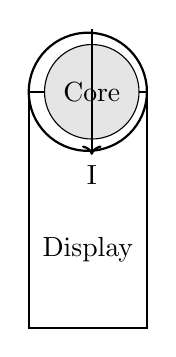
\begin{tikzpicture}
    % Body
    \draw [thick] (0,0) rectangle (1.5, -3);
    \node at (0.75, -2) {Display};
    % Clamp
    \draw [thick] (0,0) arc (180:0:0.75) -- (1.5,0); % Top arc
    \draw [thick] (0,0) arc (180:360:0.75); % Bottom of clamp ring logic
    % Better drawing
    \draw [fill=gray!20] (0.2, 0) arc (180:0:0.6) -- (1.4, 0); 
    \draw [fill=gray!20] (0.2, 0) arc (180:360:0.6) -- (1.4, 0);
    \node at (0.8, 0) {Core};
    \draw [thick, ->] (0.8, 0.8) -- (0.8, -0.8) node[below] {I}; % Conductor
\end{tikzpicture}
\captionof{figure}{Clamp Meter}
\end{center}

\textbf{Working}:
\begin{itemize}
    \item Current carrying conductor acts as single-turn primary of transformer.
    \item Clamp core acts as magnetic core.
    \item Induces voltage in secondary coil inside meter.
    \item Voltage proportional to current.
\end{itemize}
\end{solutionbox}

\begin{mnemonicbox}
\mnemonic{CLIP - Clamp measures current, Lets magnetic Induction Produce voltage}
\end{mnemonicbox}

\questionmarks{5(c) OR}{7}{Explain the working principle of a digital IC tester. Describe its block diagram and explain how it is used to test the functionality of digital ICs with a suitable example.}

\begin{solutionbox}
\textbf{Digital IC Tester}: Verifies IC functionality by truth table comparison.

\textbf{Block Diagram}:
\begin{center}
\begin{tikzpicture}[node distance=1.5cm, auto]
    \node [gtu block] (Micro) {Microcontroller};
    \node [gtu block, right=of Micro] (Patt) {Pattern Gen};
    \node [gtu block, right=of Patt] (ZIF) {ZIF Socket};
    \node [gtu block, below=of ZIF] (Resp) {Response Analyzer};
    \node [gtu block, left=of Micro] (UI) {Keypad/Disp};
    \node [gtu block, above=of ZIF] (PS) {Power Supply};
    
    \draw [gtu arrow] (UI) -- (Micro);
    \draw [gtu arrow] (Micro) -- (Patt);
    \draw [gtu arrow] (Patt) -- (ZIF);
    \draw [gtu arrow] (ZIF) -- (Resp);
    \draw [gtu arrow] (Resp) -| (Micro);
    \draw [gtu arrow] (PS) -- (ZIF);
\end{tikzpicture}
\captionof{figure}{Digital IC Tester}
\end{center}

\textbf{Working}:
\begin{enumerate}
    \item \keyword{Test Pattern Memory}: Stores truth tables for various ICs.
    \item \keyword{ZIF Socket}: Holds the IC under test.
    \item \keyword{Pattern Generator}: Applies inputs (0s and 1s) to IC pins.
    \item \keyword{Analyzer}: Reads outputs and compares with expected values.
\end{enumerate}

\textbf{Example (7400 NAND)}:
\begin{itemize}
    \item Apply 0,0 $\rightarrow$ Expect 1.
    \item Apply 1,1 $\rightarrow$ Expect 0.
    \item If difference found $\rightarrow$ Fail. Else $\rightarrow$ Pass.
\end{itemize}
\end{solutionbox}

\begin{mnemonicbox}
\mnemonic{TEST - Test patterns Exercise all States, Then verify outputs}
\end{mnemonicbox}

\end{document}




